%% LyX 2.2.2 created this file.  For more info, see http://www.lyx.org/.
%% Do not edit unless you really know what you are doing.
\documentclass[english,aps,prd,tightenlines,superscriptaddress,nofootinbib,showpacs,showkeys,floatfix,twocolumn]{revtex4}
\usepackage[latin9]{inputenc}
\setcounter{secnumdepth}{3}
\usepackage{color}
\usepackage{hyperref}
\usepackage{verbatim}
\usepackage{amsmath}
\usepackage{amssymb}
\usepackage{graphicx}
\PassOptionsToPackage{normalem}{ulem}
\usepackage{ulem}

\makeatletter

%%%%%%%%%%%%%%%%%%%%%%%%%%%%%% LyX specific LaTeX commands.
%% Because html converters don't know tabularnewline
\providecommand{\tabularnewline}{\\}

%%%%%%%%%%%%%%%%%%%%%%%%%%%%%% Textclass specific LaTeX commands.
\@ifundefined{textcolor}{}
{%
 \definecolor{BLACK}{gray}{0}
 \definecolor{WHITE}{gray}{1}
 \definecolor{RED}{rgb}{1,0,0}
 \definecolor{GREEN}{rgb}{0,1,0}
 \definecolor{BLUE}{rgb}{0,0,1}
 \definecolor{CYAN}{cmyk}{1,0,0,0}
 \definecolor{MAGENTA}{cmyk}{0,1,0,0}
 \definecolor{YELLOW}{cmyk}{0,0,1,0}
}

%%%%%%%%%%%%%%%%%%%%%%%%%%%%%% User specified LaTeX commands.
\PassOptionsToPackage{english}{babel}

\usepackage{float}
\usepackage{mathrsfs}
\usepackage{amsfonts}
\usepackage{array}
\usepackage{epsfig}
% need for subequations
% defines \lesssim, etc
\usepackage{graphicx}% need for figures
\usepackage{verbatim}% useful for program listings
% use if color is used in text
%\linespread{1.5}

\renewcommand{\thefootnote}{\fnsymbol{footnote}}
\def\ltap{\raisebox{-.6ex}{\rlap{$\,\sim\,$}} \raisebox{.4ex}{$\,<\,$}}
\def\gtap{\raisebox{-.6ex}{\rlap{$\,\sim\,$}} \raisebox{.4ex}{$\,>\,$}}
\def\lra{\leftrightarrow}
\def\naive{na\"{\i}ve}
\newcommand{\as}{\alpha_{\mathrm{S}}}
\newcommand{\f}[2]{\frac{#1}{#2}}
\def\beq{\begin{equation}}
\def\b0{\beta_0}
\def\bone{\beta_1}
\def\btwo{\beta_2}
\def\eeq{\end{equation}}
\def\beeq{\begin{eqnarray}}
\def\eeeq{\end{eqnarray}}
\def\bom#1{{\mbox{\boldmath $#1$}}}
\def\to{\rightarrow}
\def\ito{\leftarrow}
\def\nn{\nonumber}
\def\arrowlimit#1{\mathrel{\mathop{\longrightarrow}\limits_{#1}}}
\def\qt{q_T}
\newcommand{\asFPi}{\frac{\as}{4\pi}}
\def\ptmin{p_{T{\rm min}}}
\def\ptmax{p_{T{\rm max}}}
\def\ms{${\overline {\rm MS}}$}
\def\tL{{\widetilde L}}
\newcommand{\ib}{\bar{\imath}}

\makeatother

\begin{document}

\title{PDFSense: A tool for exploring the sensitivity of hadronic experiments to nucleon structure}

\author{Bo Ting Wang}
\email{botingw@smu.edu}


\affiliation{Department of Physics, Southern Methodist University,\\
 Dallas, TX 75275-0181, U.S.A. }

\author{Sean Doyle}
\email{seand@smu.edu}


\author{Jun Gao}

\affiliation{School of Physics and Astronomy, INPAC,\\
 Shanghai Key Laboratory for Particle Physics and Cosmology,\\
 Shanghai Jiao-Tong University, Shanghai 200240, China}
\email{jung49@sjtu.edu.cn}


\affiliation{ Department of Physics, Southern Methodist University,\\
 Dallas, TX 75275-0181, U.S.A. }

\author{T.~J.~Hobbs}
\email{tjhobbs@smu.edu}


\affiliation{Department of Physics, Southern Methodist University,\\
 Dallas, TX 75275-0181, U.S.A. }

\author{Tie-Jiun Hou}
\email{tiejiun.hou@foxmail.com}


\affiliation{School of Physics Science and Technology, Xinjiang University,\\
 Urumqi, Xinjiang 830046 China }

\author{Pavel Nadolsky}
\email{nadolsky@smu.edu}


\affiliation{ Department of Physics, Southern Methodist University,\\
 Dallas, TX 75275-0181, U.S.A. }

\author{Fredrick I. Olness}
\email{olness@smu.edu}


\affiliation{ Department of Physics, Southern Methodist University,\\
 Dallas, TX 75275-0181, U.S.A. }
\begin{abstract}
We demonstrate a collection of tools and metrics for quantitatively
studying the sensitivity of hadronic measurements to the underlying
Parton Distribution Functions (PDFs). \\
 \\
 \textcolor{red}{Replace PACS with PhySH:}\texttt{\textcolor{red}{https://www.aps.org/publications/apsnews/201602/classification.cfm}} 
\end{abstract}

\pacs{\textcolor{red}{12.15.Ji, 12.38 Cy, 13.85.Qk}}

\keywords{parton distribution functions; large hadron collider; Higgs boson}

\maketitle
\newpage{}\tableofcontents{}\newpage{}

\section{Introduction}
%
The determination of the collinear parton distribution functions (PDFs) of the nucleon
has increasingly become a precision discipline in recent years with the advent of
high statistics programs at both fixed-target experiments and colliders.
%
%\textcolor{red}{We'll polish this part near the end}
%
% \subsection{Statement of the Problem}
%
Parton distribution functions (PDFs) are crucial for understanding
the behavior of hadron collisions and then exploring the Standard
Model (SM). PDFs describe the structure of hadrons, which affect the
configurations of the final particles in the collisions. Therefore,
the magnitudes of physical observables in hadron collisions strongly
depend on PDFs. Currently, The Large Hadron Collider (LHC) produces
a lot of experimental data. Owning to the fact that uncertainties
in measurements constantly decrease, reducing the PDF uncertainties
of physical observables and using the higher order PDFs will make
it easier to find the inconsistency between SM and the data sets collected
by the LHC and then discover new physics. Incorporating more (LHC)
new data sets in the global fits of PDFs is a naive way to generate
better PDF sets with small uncertainties.

However, incorporating more experimental data points will substantially
increase the time for fitting PDF sets, especially when we fit higher
order PDF sets. From here we know that how to select data sets in
global fits will become extremely important in the near future. It
is essential to know which data sets will effective constrain the
higher order PDFs for the global fits in the limited time of computation.
In addition, because physical predictions are sensitive to respective
flavors and regions of $\{x,\mu\}$ in PDFs, we need to narrow
down uncertainties of the specific regions of $\{x,\mu\}$ (in the
PDFs). Where partonic $x$ are momentum fractions and $\mu$ are
QCD factorization scales. For example, if PDF values for the leading
$\{x,\mu\}$ ranges and flavors that characterize kinematical quantities
for Higgs production processes (e.g. at $\mu=125$ GeV) are tightly
constrained, the theoretical predictions for these processes are reliable
(precise).
%\begin{enumerate}
%\item methods

Using correlation between PDF uncertainties in two observables have
been proposed to study constraints on PDFs and constraints on observables
imposed by PDFs \cite{Pumplin:2001ct}\cite{Nadolsky:2001yg}\cite{Nadolsky:2008zw}. 
%\item the evaluation of the methods

The approach can help us to find the $\{x,\mu\}$ ranges of PDFs
affecting physical observables such as total cross section \cite{Nadolsky:2008zw}.
It is yet be established that how to know the ranges specifying PDFs
constrained by experimental data sets. 
%\end{enumerate}

%\subsection{Objectives}

Thus, establishing a better understanding of the relationships between
the strength of constraints on PDF and experimental data sets will
be a significant and beneficial contribution to particle physics.

%\subsection{Methodology}

We have developed and tested a systematic method to study the constraints
on PDFs imposed by the experimental data sets. We will use established
statistical observables to quantify the strength of these constraints.

After that, we introduce a new statistical package {\it PDFSense} to visualize
the regions of partonic momentum fractions $x$ and QCD factorization
scales $\mu$ where the experiments impose strong constraints on the
PDFs. Recent experimental data will be considered in the analysis
in order to provide better constraints to various ranges of PDFs.
%
%\begin{enumerate}
%\item Scope, Limitations and Assumptions 
%\item Significance 
%\item Structure of This Paper 
%\end{enumerate}

%\subsection{Overview of paper}

The remainder of the article proceeds as follows.
Essential details regarding the PDFs and their standard determination via QCD global
analyses are summarized in \ref{sec:pdfs}.
The basic statistical ingredients of our analysis are presented in Sec.~\ref{sec:pdfsense},
along with an introduction to 
our analysis package {\it PDFSense}.
To highlight the utility of the resulting framework, we perform an assessment of the potential
impact of hypothetical LHeC pseudodata in Sec.~\ref{sec:lhec}; in the conclusion contained
in Sec.\ref{sec:conc} we emphasize a number of physics insights that may be gained with
{\it PDFSense}, while a number of statistical details and supporting figures and
tables are reserved for Apps.~\ref{sec:stats} and \ref{sec:supp}, respectively.

%\section{Overview of Global fitting and Constraints on PDFs }
\section{PDF preliminaries}
\label{sec:pdfs}
%
While various theoretical methods exist to compute nucleon PDFs in terms of models,
their unambiguous evaluation in terms of QCD is not yet possible due to the fact that
the PDFs can in general receive substantial nonperturbative contributions at infrared
momenta. For this reason, precise PDF determination has proceeded mainly through the
technique of QCD global analysis --- a method enabled by the QCD factorization theorem.

In this approach, a highly flexible parametric form is ascribed for the various flavors
in a given analysis at a relatively low scale $Q^2_0$. For example, in the commonly used Hessian
Method one might take the input PDF for a given quark flavor $f$ according to be an $n$-parameter form
%
\begin{equation}
f(x,Q_{0}^{2})=a_{f0}\,x^{a_{f1}}(1-x)^{a_{f2}}\,F(a_{f3}, \dots, a_{fn})\ ,
\label{eq:fitform}
\end{equation}
%
in which $F(a_{f3}, \dots, a_{fn})$ is typically a suitable polynomial function,
{\it e.g.}, a Chebyshev polynomial.
%
In this circumstance, a best fit is then found for the parameters $a_{f0}$, \dots, $a_{fn}$
by minimizing a $\chi^{2}$ function with respect to the world's data for which physical
observables can be computed in terms of the PDFs by the factorization theorem; the resulting
uncertainties are determined by requiring that the $\chi^{2}$ function remain appropriately
small under minor perturbations of the fit parameters $\{ a_{fn} \}$ subject to the condition
%
\begin{equation}
\chi^{2}\, <\, \chi_{min}^{2}+\chi_{torelance}^{2}\ .
\end{equation}
%
From this information it is then possible to convert from a parametric basis
$\{ a_{fn} \}$ basis to a basis of eigenvectors $\{r_{i}\}$ in terms of which
a set of PDF error replicas may be generated that encapsulate the constraint
to the proton PDFs from the world's data.


Due to the presence of correlated systematic errors in many experimental
data sets, it should be noted that the most appropriate $\chi^{2}$ function
is in general
%
\begin{align}
\label{eq:chi2}
	\chi^{2} &= \sum_i\, r^2_{i,\,shift}\, +\, \sum^K_{k=1} \rho^2_k \\
%
	r_{i,\,shift} & ={1 \over \sigma_{i}}\, \big( T_{i}-D_{i,\,shift} \big)\ ,
\label{eq:residual}
\end{align}
%
where the sum over $i$ accounts for the individual data points in the set of
global data, and $r_{i,\,shift}$, $T_{i}$, and $\sigma_{i}$ are the {\it residual},
theoretical prediction evaluated in terms of PDFs, and total uncorrelated
uncertainty for the $i^{th}$ data point, respectively. On the other hand, $D_{i,\,shift}$
represent the central values of the experimental data, shifted to incorporate
the effect of systematic correlations as described in App.~B of Ref.~\cite{Pumplin:2002vw},
with $\rho_k$ in Eq.~(\ref{eq:chi2}) the random shift parameters associated with
$K$ sources of correlated systematic error. We henceforth refer to the residuals
corresponding to data shifted with respect to correlated errors simply as $r_i$
for compactness.


In consequence of these defintions, both the residual $r_{i}$ and $\chi^2$
may be thought of as broadly characterizing the quality of a given fit
to a large data set, with the scenario $\chi^{2}\gg N_{data}$ implying
a poor fit, whereas $\chi^{2}\leq N_{data}$ is consistent with a
strong description of the data. At the same time, fits that too sharply
limit $\chi^{2}\ll N_{data}$ correspond to an overfit of the data.


%We assume good fits are theoretical predictions within experimental error bar.
%We can estimate
%the goodness of the fit of this point.
%For data sets, the goodness
%of fits is the sum of all points $i$ and $r_{i}$, which means that
%we use the squared distance to evaluate the agreement between the
%model and the data sets. Hence, we can obtain the best coefficients
%of the model by minimizing $\chi^{2}$. If $\chi^{2}\gg N_{data}$
%for a data set and a theory, this fit is bad. If $\chi^{2}\leq N_{data}$,
%this fit is better than expected. If $\chi^{2}\ll N_{data}$, this
%fit is over-fitted. To sum up, $r_{i}$ and $\chi^{2}$ could be defined
%as follows:
%
%Here we provide criteria of good PDF fittings 
%%
%%\begin{enumerate}
%...$\chi^{2}\simeq N_{data}$, the smaller a $\chi^{2}$, the better
%a fitting 
%%
%...if residuals of points $i$ are small ($|r|<1$, $r$ is called residual
%$\frac{T_{i}-D_{shift,i}}{\sigma_{i}}$), the fit of these points
%is good$\sum_{f}\ f\,(x,\mu^{2})$= 1
%\end{enumerate}


%In general, we estimate the uncertainties of the parameters describing
%PDFs by constraining $\chi^{2}$ value. In other words, we identify
%the region representing to the parameter uncertainties by the region
%with $\chi^{2}$ smaller than $\chi_{min}^{2}+\chi_{torelance}^{2}$.
%We learn that constraints on PDFs are from constraining the upper
%bound of the goodness of fits. When we fit theoretical models to match
%experimental data so that $r_{i}$ for data points $i$ and $\chi^{2}$
%are not too large, PDFs are constrained. Thus, we use $\chi^{2}$
%and $r_{i}$ to see the constraints on PDFs because they represent
%the criteria of the goodness of fits and $f_{a}(x,\mu)$ values
%are constrained to meet this criteria. In other words, the criteria
%could determine the range of $f_{a}(x,\mu)$.





%\end{enumerate}
%\sout{To fit PDF sets, we first need to determine the input theoretical
%model and data sets. The model includes the selection of quark mass,
%coupling constants and the order considered in the correction of perturbation
%(i.e. LO, NLO and etc). Then we determine the parametrization function
%form $f_{q}(x,Q_{0})=a_{0}x^{a_{1}}(1-x)^{a_{2}}F(a_{3},a_{4},......)$
%at the lowest factorization scale $Q_{0}$, for which we need to take
%some physical rules into account. For instance, $a_{0}x^{a_{1}}(1-x)^{a_{2}}$
%term requires that the probabilities of the partons with momentum
%fraction $x=1$ or $x=0$ are $0$. Besides, the momentum conservation
%($\int_{0}^{1}x\underset{i}{\sum}f_{i}(x,Q)dx=1$) requires that
%the total momentum of all subparticles in each hadron should equal
%to the kinematical momentum of that hadron. ($\int_{0}^{1}(u(x)-\bar{u}(x))dx=2$
%and $\int_{0}^{1}(d(x)-\bar{d}(x))dx=1$) require that protons consist
%of $uud$ at the low factorization scale. we use $\chi^{2}$ minimization
%to explore the best fit parameters $a_{0}$, $a_{1}$, $a_{2}$ and
%etc. $\chi^{2}$ analysis applies the ratios of the deviations between
%theoretical predictions and experimental values to experimental error
%bars to quantify the goodness of fits. Here are steps of the PDF fitting: }

...select the experimental data sets and theoretical model in
global fits 
%
...write down parametrization functions of all flavors 
%
...determine the best-fitted $a_{0}$, $a_{1}$, $a_{2}$......
of the parametrization functions by minimizing $\chi^{2}$ 
%
determine uncertainties of the parametrization functions
by requiring $\chi^{2}<\chi_{min}^{2}+\chi_{torelance}^{2}$


\section{PDFSense}
\label{sec:pdfsense}
%
%\textcolor{red}{framework}
%
\onecolumngrid


% % % % % FIG_1
%
\begin{figure}[h]
\includegraphics[width=1.0\textwidth]{figs/xQbyexpt_xQ.pdf}
\caption{
	A graphical representation in $(x,\mu)$ space of the full dataset treated in the present analysis, essentially corresponding to
	an expansion of the data fitted in the most recent
	CT14 analysis, which included fixed-target measurements from Run II of HERA as described in
	Ref.~\cite{Hou:2016nqm} (CT14HERA2); we take this data set to be the default in the present analysis and illustrate
	the potential of {\it PDFSense} to illustrate the differential impact of the separately labeled
	data sets represented here in PDF determinations, with the CT14HERA2 PDF set as an illustrative example.
	We note that the points are labeled according to experimental ID number; a detailed translation key
	to individual experiments is given in Tables~\ref{tab:EXP_1}--\ref{tab:EXP_3}
}
\label{fig:data}
\end{figure}
\twocolumngrid

We have developed and tested a systematic method to study the constraints
on PDFs imposed by experimental data sets. We use established statistical
observables to quantify the strength of these constraints. After that,
We introduce a statistical technique to visualize the regions of partonic
momentum fractions $x$ and QCD factorization scales $\mu$ where
the experiments impose strong constraints on the PDFs. Recent experimental
data is considered in the analysis in order to provide better constraints
to various ranges of PDFs.

To test the effectiveness of the proposed method, we study constraints
on CT14HERA2 parton distributions \cite{Hou:2016nqm} from various
data sets. We include various types of experimental data sets in the
analysis, including DIS processes, $Z\rightarrow l^{+}l^{-},d\sigma/dy(l)$,
$W\rightarrow l\nu$, and jet productions ($p_{1}p_{2}\rightarrow jjX)$.



For data sets of interest, we can demonstrate and identify values
of correlation/sensitivity data by different colors on the $x-\mu$
plane ($2D-x-\mu$ figure), such as Figs. \ref{fig:sensitivity},
which help us to rapidly estimate the distribution of the strength
of constraints on the $x-\mu$ plane. We can also know the number
of data points constraining PDFs by the histograms of the statistical
quantities.

\subsection{Statistical definitions}
\label{subsec:Sensitivity-data-PDF}
%
%\textcolor{red}{introduction correlation and sensitivity}
%
Among various quantities that characterize the impact of
experimental data upon the PDFs, the correlations, which we define
according to
%
\begin{equation}
	c^i_f (x, \mu)\, \equiv\, Corr[ f(x,\mu),r_{i} ]\ ,
\label{eq:corr}
\end{equation}
%
encodes the quantitative relation between the PDFs $f(x,\mu)$ and residuals $r_{i}$, and can determine whether
there exist predictive relationships between PDFs and goodness of
fit to data points. The formal definition and origin of the correlation of Eq.~(\ref{eq:corr})
is given in detail in App.~\ref{sec:stats}.
%
% We can also define a factor $\delta r_{i}\times Corr(f_{a}(x,\mu),r_{i})$
% to quantify the sensitivity of the experimental datum to a variation
% of the PDF. Both correlation and sensitivity are useful for constraining
% PDFs. 


Correlation illustrates the strength of the predictive relation between
any two observables $X$ and $Y$. We can use values of one observable
to predict values of another observable very well when their correlation
is close to $\pm1$. correlations of Hessian uncertainties \cite{Pumplin:2001ct}
have been used to see the simultaneous constraint on observables $X$
and $Y$, and to get constraints on PDFs \cite{Pumplin:2001ct,Nadolsky:2001yg,Nadolsky:2008zw}.
First, via measuring one physical observable, we are able to predict
the value of another observable precisely. In addition, strong correlations
are highly likely to show the signs of some physical relations, such
as causation, between the two observables.

%\textcolor{red}{Hessian correlation: definition and physical meaning}

While the correlation $c^i_f (x, \mu)$ can provide insight into the relationship between the $x$, $\mu$
dependence of a set of PDFs and associated PDF uncertainty, it alone does not fully quantify the
extent to which individual data points constrain fit uncertainties; similarly, the correlation alone
does not encode by itself the potential impact of separate or new measurements in improving PDF
determinations in terms of uncertainty reduction. For this purpose, we define the {\it sensitivity}
of the $i^{th}$ data point to the PDF of flavor $f$,
%
\begin{equation}
	s^i_f\ \equiv\ {\delta^{(\mathrm{PDF})} r_i \over \sqrt{\frac{1}{N} \sum^N_{i=1} r^2_i}}\, c^i_f(x,\mu)\ ,
\label{eq:sens}
\end{equation}
%
where the sum is up to $N$, which we take to be the total number of data points in a given experimental data set.
In Eq.~(\ref{eq:sens}), the quantity $\delta^{(\mathrm{PDF})} r_i$ represents the variation of the residuals
accross the set of Hessian error PDFs, which we normalize the quadrature-summed residual for a given experiment.
This definition has the benefit of encoding not only the correlated relationship between the PDF at a given
$(x,\mu)$ with the residual, but also the comparative size of the experimental uncertainty with respect to
state-of-the-art PDF uncertainties. In consequence, for example, new experimental data with reported uncertainties much
tighter than present PDF errors would register as high sensitivity points by the definition in Eq.~(\ref{eq:sens}).
Fig.~\ref{fig:deltaR} and the associated discussion in App.~\ref{sec:stats} describe this point theoretically, and
we illustrate this behavior with a number of practical examples below.


There are several ways to evaluate uncertainties on PDFs such as the
Hessian method \cite{Pumplin:2001ct}, the Monte Carlo method \cite{Giele:1998gw}\cite{Giele:2001mr},
and the Lagrange Multiplier \cite{Stump:2001gu}. Our PDF set input
is CT14HERA2, which uses the Hessian method to estimate uncertainties
information. This idea is based on the quadratic assumption. According
to the quadratic assumption, we will get an elliptical shape of PDF
parameter space around the best fit parameters $\overset{\rightharpoonup}{a_{0}}$
for a given tolerance parameter $\chi_{tolerance}^{2}$ satisfying
$\chi^{2}(\overset{\rightharpoonup}{a})<\chi^{2}(\overset{\rightharpoonup}{a_{0}})+\chi_{torelance}^{2}$.
If errors of an observable $X$ along the $\pm$ directions of $i$-th
dimension of the ellipse are $X_{i}^{+}$ and $X_{i}^{-}$, the uncertainty
of $X$ based on the variation of parameter at $i$-th dimension could
be approximated by $(X_{i}^{+}-X_{i}^{-})/2$. According to the principle
of error propagations, the $X$ uncertainty via PDF parameter space
is $\Delta X=\frac{1}{2}\sqrt{\underset{i}{\sum}(X_{i}^{+}-X_{i}^{-})^{2}}$.

\textcolor{red}{Move these definitions to an appendix???}

Our idea of studying PDF constraints from data sets uses the correlation
between PDF Hessian sets and residual Hessian sets, where the Hessian
correlation of two observables is defined as $cos\phi=\underset{i}{\sum}(X_{i}^{+}-X_{i}^{-})(Y_{i}^{+}-Y_{i}^{-})/4\Delta X\Delta Y$.
The correlation of any two observables $X$ and $Y$ could be used
to see the simultaneous constraint of $X$ and $Y$ \cite{Pumplin:2001ct}.
The ellipse of simultaneous constraint could be described by Lissajous
figure

\[
X=X_{0}+\Delta X\,sin(\theta+\phi)
\]

\[
Y=Y_{0}+\Delta Y\,sin(\theta+\phi)
\]
where $0<\theta<2\pi$ traces the shape of the ellipse, and whether
the shape is needle-like or circle-like is controlled by $\phi$.
If $|cos\phi|\simeq1$, the shape is needle-like, which strongly constrains
$Y$ for a given $\delta X$ (see Fig. \ref{fig:corr-ellipse}). Thus,
the correlations $Corr(f_{a}(x,\mu),r_{i})$ of PDFs $f_{a}(x,\mu)$
and the residuals $r_{i}$\textcolor{black}{{} }can determine the
strength of constraints on PDFs imposed by $r_{i}$ in experimental
data points. 

% \textcolor{red}{construct more representative statistical quantity
% for constraints: }

strength of constraints on PDFs imposed by $r_{i}$ ($SOC(PDF)$)

Although we can know the predictivities between PDFs and measurements
through $Corr(f_{a}(x,\mu),r_{i})$, $Corr(f_{a}(x,\mu),r_{i})$
could not specify the strength of constraints on PDFs imposed by $r_{i}$
($SOC(PDF)$). For instance, the measurements with large uncertainties
cannot effectively constrain $f_{a}(x,\mu)$ no matter how large
$Corr(f_{a}(x,\mu),r_{i})$ is, since $r_{i}$ is not sensitive
to the variation of $f_{a}(x,\mu)$. Therefore, we want to find
a more representative statistical quantity for $SOC(PDF)$. \textcolor{black}{To
study }$SOC(PDF)$\textcolor{black}{{} between PDFs and data sets,
we study the variation of }$\chi^{2}$\textcolor{black}{{} and }$r_{i}$\textcolor{black}{{}
associated with the fluctuation in }$f_{a}(x,\mu)$\textcolor{black}{.
Fig. \ref{fig:sensitivity} shows }$r_{i}$\textcolor{black}{{} in
data points depending on the variation in }$f_{a}(x,\mu)$\textcolor{black}{{}
error sets. We find that despite the fact that the correlation between
}$r_{i}$\textcolor{black}{{} in two data points (red circles and
blue circles) and }$f_{a}(x,\mu)$\textcolor{black}{{} are the
same, the fluctuation for }$f_{a}(x,\mu)$\textcolor{black}{{}
imposes different levels of impact to }$r_{i}$.\textcolor{black}{{}
The }$r_{i}$,\textcolor{black}{{} represented by red circles, are
more sensitive to }$f_{a}(x,\mu)$\textcolor{black}{, which indicates
that when we constrain }$\chi^{2}$\textcolor{black}{{} for getting
the new fitted }$f_{a}(x,\mu)$\textcolor{black}{{} error sets,
the data point represented by the red circles will more dramatically
narrow down the range of the new }$f_{a}(x,\mu)$\textcolor{black}{{}
error sets so that }$r_{i}$\textcolor{black}{{} for error sets become
smaller. Here we find the }$\delta r_{i}$\textcolor{black}{, which
evaluates the fraction of theoretical and experimental uncertainties,
indicating whether the theoretical uncertainties are apt to be constrained
after the fitting. For the above reasons, we advise using }$\delta r_{i}\times Corr(f_{a}(x,\mu),r_{i})$\textcolor{black}{{}
to quantify the sensitivity (}$Sen(f_{a}(x,\mu),r_{i})$\textcolor{black}{)
for }$r_{i}$\textcolor{black}{{} to }$f_{a}(x,\mu)$\textcolor{black}{,
and using the sensitivity to estimate }$SOC(PDF)$\textcolor{black}{{}
for data point }$i$\textcolor{black}{. }

\subsection{Correlation and Sensitivity analysis}
\label{subsec:main-demo}
%
Having outlined the main statistical quantities of interest in the preceding
subsection, we turn now
to their implementation in the correlation and sensitivity analysis package
{\it PDFSense}. As described in the previous sections, our aim is to quickly
evaluate the impact of various hadronic data sets upon the present knowledge
of the PDFs in a fashion that does not require a full QCD analysis of the
type described in Sec.~\ref{sec:pdfs}. As a demonstration of how {\it PDFSense}
achieves this, we treat the data set shown in Fig.~\ref{fig:data} of the most recent NNLO CT14 analysis of the
global data set augmented by the HERA Run II fitted in Ref.~\cite{Hou:2016nqm}
(which we refer to as CT14HERA2),
explicitly showing how various constituent data sets constrain PDFs in a full
space of $(x, \mu)$. We have already noted the magnitude of this data set, which
is decomposed into separate experiments in Fig.~\ref{fig:data}.


%\onecolumngrid


%
% % % % % % % % % % % % % % % % % % % % % % % % % % % % % % % % % % % % 
% % % FIG_2
\begin{figure}
\includegraphics[clip,width=0.43\textwidth]{figs/corr_hist+1_f0_samept}
\includegraphics[clip,width=0.493\textwidth]{figs/corr_xQ+1_f0_samept}
\caption{
	Two representations of the correlation $c^i_g(x,\mu)$ of the gluon PDF $g(x,\mu)$
	with the pointwise residual $r_i$ of the CT14HERA2 analysis; in the upper panel we plot a
	histogram showing the distribution of correlations over 5010 points. In the lower panel 
	we show the $(x,\mu)$ map of these correlations as produced by {\it PDFSense} for the full data set.
	}
\label{fig:corr-main}
\end{figure}

% % % FIG_3
\begin{figure}
\includegraphics[clip,width=0.43\textwidth]{figs/corrdr_hist+1_f0_samept}
\includegraphics[clip,width=0.493\textwidth]{figs/corrdr_xQ+1_f0_samept}
\caption{
	Like Fig.~\ref{fig:corr-main}, but for the gluon sensitivity
	$s^i_g(x,\mu)$ as defined in Eq.~(\ref{eq:sens}).
}
\label{fig:sens-main}
\end{figure}
%
% % % % % % % % % % % % % % % % % % % % % % % % % % % % % % % % % % % % 
%


%\twocolumngrid


In principle, we can use the correlation \& sensitivity mentioned
above to quantify $SOC(PDF)$ for any points on the $x-\mu$ plane
and data point $i$. Therefore, we can identify which regions in the
$x-\mu$ plane have strong $SOC(PDF)$. Our objective is to characterize
the strongly constrained ranges (Strong $SOC(PDF)$ Regions) imposed
by the given data sets.


Given its centrality in many PDF analyses, we concentrate our demonstration in
the present section upon the gluon distribution, $g(x,\mu)$. In fact, the gluon
PDF remains dominated by substantial uncertainties at both $x \sim 0$ and in 
the elastic limit $x \to 1$, a fact which has driven an intense focus upon,
{\it e.g.}, top quark and jet production processes at colliders, which themselves
are typically measured at large center-of-mass energies $\sqrt{s}$ where the
dependence upon the low $x$ behavior of the gluon distribution is especially
relevant.


We first consider plots of the correlations for the gluon distribution, both
as a histogram and as fully represented in a space of $(x,\mu)$.
A striking feature of the correlation plot is the large magnitude found for
the inclusive jet production measurements (inverted triangles) for which large
gluon-residual correlations $c_g(x,\mu) > 0.85$ are found, especially at the
highest values of $x$ and $\mu$ represented in Fig.~\ref{fig:corr-main}.

We can also consider the analogous plot for the sensitivity of the data
to the gluon distribution, which we plot in Fig.~\ref{fig:sens-main}.
Here, an evident feature is the comparitive reduction of the ``temperature''
of the plot due to the inclusion of $\delta^{(\mathrm{PDF})} r_i$ in the
defintion of the sensitivity. In reasonable agreement with expectation,
we also observe the most heightened sensitivities for the points
at lowest $x$ --- especially for the combined HERA data set ---
in accord with the fact that PDF errors for the gluon distribution
are in general least controlled at these $x$ ranges.


%\textcolor{red}{difficulties in the analysis and solutions}
%
%Acquiring the corresponding Strong $SOC(PDF)$ Regions for each point
%$i$ still could not tell us which ranges are constrained by each
%data set because the amount of information in all data points is too
%large to analyze it. Therefore, we present a simple method as follows.
%For each data point $i$, we select the points (or the ranges) in
%the $x-\mu$ plane whose $f_{a}(x_{i},\mu_{i})$ are constrained
%most by the point $i$ (Max $SOC(PDF)$ Regions). Here we assume that
%in scattering processes, sizes of physical observables are mainly
%contributed by the ranges near $\{x_{i},\mu_{i}\}$. Thus, it is
%highly possible that the measurement at point $i$ will impose the
%strongest constraints on the $f_{a}(x_{i},\mu_{i})$ in these ranges.
%As a result, the combination of these ranges describes the most constrained
%ranges for all data points in each data set.
%
%\textcolor{red}{capability}
%
%It is possible to evaluate those PDF ranges. For each experimental
%data point $i$, we can establish an approximate relation between
%the kinematical quantities for that data point, and unobserved quantities
%$a$, $x$, and $\mu$ specifying the PDFs, where $a$, $x$,
%and $\mu$ are flavor, momentum fraction, and resolution scale of
%partons. For example, in DIS, $x$ and $\mu$ are approximately
%equal to Bjorken $x$ and momentum transfer $Q$ according to the
%Born-level kinematic relation. However, this relation is violated
%in high-order radiative contributions. Nevertheless, this relation
%will approximately hold in most scattering events. Therefore, we derive
%the relation between the kinematical quantities and unobserved quantities
%we mentioned for data sets in our analysis, including DIS, $dXsec/dy(l)$
%of $Z\rightarrow l_{+}l_{-}$, $dXsec/dy(l)$ of $W\rightarrow l\nu$,
%and (di)jet productions. In practice, our fitted PDF sets are not
%perfect, so even some ranges of the real PDF dominate a physical observable,
%the PDF sets in these ranges are not always strongly correlated to
%that physical observable.
%
%Following are formulas (code part: selectExptxQv2 in %\ref{subsec:library:-dtareadbotingw2016})
%connecting experimental data points and their leading ${x,\mu}$
%points of PDFs:
%
%DIS: ${x,Q}_{data}={x,\mu}_{PDF}$
%
%$Z\rightarrow l_{+}l_{-},dXsec/dy(l)$: ${(Q/\sqrt{S})\times\exp(\pm y),Q}_{data}={x,\mu}_{PDF}$
%
%$W\rightarrow l\nu$: same as $Z\rightarrow l_{+}l_{-},dXsec/dy(l)$
%
%JP ($q_{1}q_{2}\rightarrow j_{1}j_{2}$, estimate $x_{1},x_{2}$
%of jet as peak of $y(j_{1}),y(j_{2})$): ${(2P_{T}/\sqrt{S})\times\exp(\pm y),P_{T}}_{data}={x,\mu}_{PDF}$
%
%\begin{table}
%
%\begin{tabular}{|c|c|c|c|c|}
%\hline 
%Process & Experimental  & Theortical & notes & ref???\tabularnewline
%\hline 
%\hline 
%DIS & $\{x,Q^{2}\}$ & $\{x,\mu\}$ &  & \tabularnewline
%\hline 
%Z Prog & $\{\tau,y\}$ &  &  & \tabularnewline
%\hline 
% &  &  &  & \tabularnewline
%\hline 
%Jet Pro & $\{y,p_{T}\}$ &  &  & \tabularnewline
%\hline 
%\end{tabular}\caption{table }
%
%\end{table}
%
%Here we give physics of these formulas. DIS processes are just mentioned
%in the example. In lepton pair production and (di)jet production,
%the rapidities of the final-state pairs are small for most events.
%If $y$ is integrated out, we set $y=0$ $\tau=Q/\sqrt{S}$ $x_{1}=x_{2}=\tau$.
%If $y$ of the lepton pair or jet pair is known, we set $x_{1,2}=\tau\cdot\exp(\pm y)$.
%For jet production, $\tau=2p_{T}^{{\rm jet}}/\sqrt{S}$ at the leading
%order. In most events, if rapidity $y_{l}$ of the lepton is known
%yet $y$ of the boson is unknown, we use the fact that $y_{l}\sim y\pm1$
%for most events. You can still estimate $x_{1}$ and $x_{2}$
%as $x_{1,2}=\tau\cdot\exp(\pm y)$, where $y\sim y_{l}$ (up to
%an error of less than 1 unit).
%
%\textcolor{red}{advantages}
%
%Because Max $SOC(PDF)$ Regions are obtained from a physical relation,
%we know the constraints in these ranges are the real physical constraints
%rather than the results of other factors, such as parametrization
%function dependency.
%
%\textcolor{red}{practical procedure (step by step)}
%
%Finally, we provide steps of Same point method. Steps are as follows: 
%\begin{enumerate}
%\item calculate Max $SOC(PDF)$ Regions $\{x_{i},\mu_{i}\}$ from corresponding
%experimental data points $i$ by using a suitable transformation formula
%describing the approximate relation between $\{x_{i},\mu_{i}\}$
%and kinematical quantities for points $i$ (code part: selectExptxQv2
%in XXXX) 
%\item for each data point, calculate all flavours of PDF values for the
%same $\{x_{i},\mu_{i}\}$ (executable part: fxQsamept.nb in XXXX) 
%\item calculate correlation $Corr(f_{a}(x_{i},\mu_{i}),r_{i})$, sensitivity
%$\delta r_{i}*Corr(f_{a}(x,\mu),r_{i})$, and other statistical
%quantities ($r_{i,central\,value}$, $\delta r_{i}$, and experimental
%error ratio in this code) for every point $i$ and every flavor $a$
%(executable: fxQsamept\_corr.nb in XXXX) 
%\item draw the histograms and $2D-x-\mu$ figures for the statistical
%quantities derived in step 3 (executable: run\_v3.nb in XXXX,
%example figure: XXXX) 
%\end{enumerate}
%

%\begin{figure}
%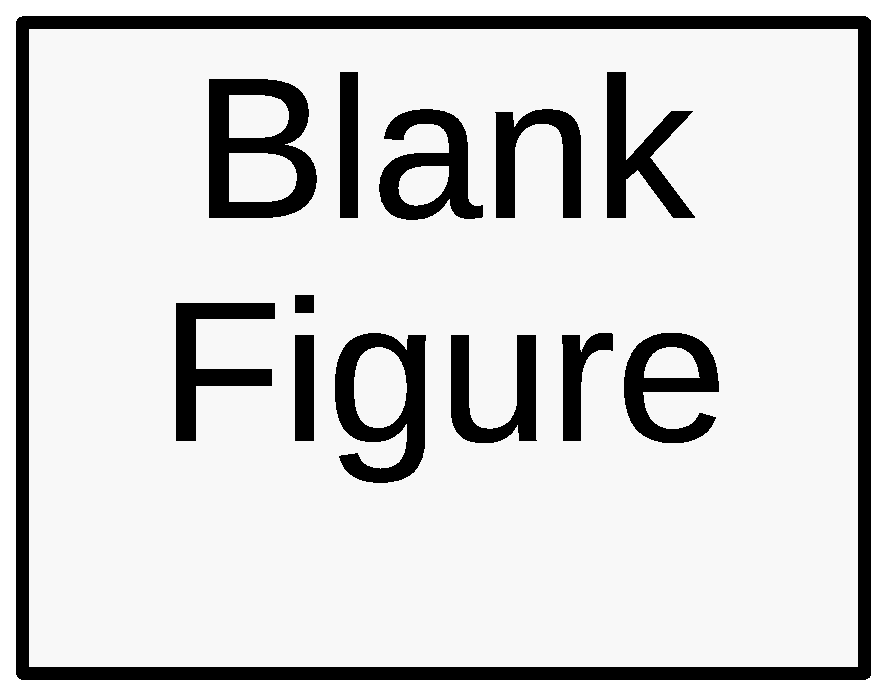
\includegraphics[clip,width=0.4\textwidth]{figs/blank}\caption{The correlation and sensitivity of the Hessian uncertainty of data
%set 247(ATL7Zpt) and CT14NNLO depending on the momentum fraction and
%the factorization scale. \label{fig:The-corr-sensitivity-247}}
%\end{figure}
%
%\begin{figure}
%\includegraphics[width=0.45\textwidth]{figs/corr_sample}\caption{Sample Figure. }
%\end{figure}
%
%\begin{figure}
%\includegraphics[width=0.45\textwidth]{figs/corr_sample}\caption{Sample Figure. }
%\end{figure}
%\cleardoublepage{}\newpage{}
%
%\section{The Metrics:}
%
%\subsection{The metrics}
%
%We briefly introduce the various metrics which we can use to evaluate
%the relative sensitivity of separate experimental measurements to
%the individual PDF flavors. 
%
%%\subsubsection{Correlations}
%
%In Figure~XXX we display the computed correlation
%between the top quark production process and the gluon PDFs. The correlations
%are defined in Eq.{*}{*}{*}{*} and the values range over the interval
%$[-1,1]$. 
%
%In Figure~XXX we show the histogram of the
%absolute values of the correlations for each of the 35 data points
%in the top quark production set. Larger magnitudes imply a stronger
%correlation, and we have arbitrarily drawn a line at $0.7$ to focus
%on the larger values. In Figure~XXX there
%are 11 out of 35 data points with an absolute correlation above the
%0.7 mark. 
%
%In Figure~XXX we display the absolute value
%of the correlation in the $\{x,\mu\}$ plane. This allows us to see
%the specific kinematic region where the data contributes. The points
%are color-coded according to the legend in the figure, and the points
%above the 0.7 threshold are enlarge to emphasize their contributions. 
%
%For $\mu\sim350\,$GeV there is a grouping of data points corresponding
%to pair production of top\textendash anti-top quarks. There is also
%a group of points {*}{*}{*} {[}describe the points on the slope{]}
%{*}{*}{*}
%
%%\subsubsection{Sensitivity}
%
%Although the correlation is a useful measure, this has a potential
%drawback that if the uncertainties of the measurement are large then
%the net constraining power of the data could be minimal. To address
%this deficiency, we can construct a new quantity which we will label
%as the sensitivity and define as the residual times the correlation.
%Thus, data sets with both a strong correlation and a strong pull will
%have a large impact on the fit, and hence a large sensitivity. 
%
%In Figure~XXX we display the computed sensitivity
%between the top quark production process and the gluon PDFs. In contrast
%to the correlations which are constrained to the interval $[-1,1]$,
%the sensitivity can in principle take on any value: $[-\infty,\infty]$;
%in practice, we expect the sensitivity to be centered about zero with
%a roughly Gaussian distribution. 
%
%In Figure~XXX we show the histogram of the
%absolute values of the sensitivity for each of the 35 data points
%in the top quark production set. Larger magnitudes imply a stronger
%sensitivity, and we have arbitrarily drawn a line at $1.0$ to focus
%on the larger values. In Figure~XXX there
%are only 1 out of 35 data points with an absolute correlation above
%the 1.0 mark. 
%
%In Figure~XXX we display the absolute value
%of the sensitivity in the $\{x,\mu\}$ plane. This allows us to see
%the specific kinematic region where the data contributes. The points
%are color-coded according to the legend in the figure, and the points
%above the 0.25 threshold are enlarge to emphasize their contributions. 
%
%Again we see the distribution of the data points are grouped along
%a line at $\mu\sim350\,$GeV corresponding to pair production of top\textendash anti-top
%quarks. There is also a group of points {*}{*}{*} {[}describe the
%points on the slope{]} {*}{*}{*}
%
% - - - - - - - - - - - - - - - - - - - - - - - - - -
%
\section{Case Study: LHeC}
\label{sec:lhec}
%
The need to disentagle, {\it e.g.}, the distribution of the gluon at low $x$ and the detailed
behavior of the light quark distributions at large $x$ (which are inherently nonperturbative)
has stimulated interest in a future high luminosity electron collider at the LHC, the
Large Hadron-electron Collider (LHeC) \cite{AbelleiraFernandez:2012cc}, which could in principle afford access to new domains
in $x$ and $Q^2$ beyond that made available by recent fixed-target or collider experiments.


Such a machine would effectively represent an analogue to HERA, albeit at substantially higher
energy and luminosity, a fact which would putatively enable it to probe various elusive phenomena, including
the onset of gluonic saturation at low $x$, diffractive effects, and, potentially, nonperturbative phenomenology
at high $x$ and heavy quark production and hadronization. The reach of this machine would in principle be especially
enhanced by the increased luminosity, which should afford a strong reduction in the size of experimental uncertainties.

To explore this possibility, we implement the pseudodata \cite{LHeCdata} generated by Klein and Radescu into {\it PDFSense} to gauge the potential
sensitivity of this information to the behavior and uncertainty of the proton PDFs as again represented by the most
recent CT14HERA2 set. For the sake of illustration, we concentrate on two banner results --- the sensitivity of the LHeC
pseudodata to the gluon distribution (shown in the top panel of Fig.~\ref{fig:LHeC}) as well as for the down quark
distribution, which we plot in the lower panel, also of Fig.~\ref{fig:LHeC}. Our plots explicitly delineate the
separate experimental channels for the pseudodata (the unpolarized reduced cross sections $\sigma^{e^\pm}_r$ for
both neutral current and charged current interactions, as accounted in the caption of Fig.~\ref{fig:LHeC}).



%\onecolumngrid


%
\begin{figure}
\includegraphics[clip,width=0.45\textwidth]{figs/LHeCH2_corrdr_xQ+1_f0_samept.pdf} \ \ \
\includegraphics[clip,width=0.45\textwidth]{figs/LHeCH2_corrdr_xQ+1_f2_samept.pdf}
\caption{
	Select sensitivity plots for the LHeC pseudodata, in this case showing $s^i_g(x,\mu)$
	in the upper panel and $s^i_d(x,\mu)$ in the lower. The pseudodata are broken among four separate
	reaction channels --- CC $e^- p$ (circles) and $e^+ p$ (squares) as well as NC $e^- p$ (diamonds)
	and $e^+ p$ (triangles).
	}
\label{fig:LHeC}
\end{figure}



%\twocolumngrid



%
% - - - - - - - - - - - - - - - - - - - - - - - - - -
%
%
%Using the correlations and the sensitivity described in the previous
%chapter, we can examine individual data sets to answer detailed questions
%about the influence on the PDF flavors. 
%
%Here we will present two example analyses demonstrating the utility
%of these metrics. First we will study the influence of both the top
%quark and jet production data on the gluon PDF. Next we will look
%at a future LHeC facility and investigate how new data might further
%constrain the PDFs. 
%
%\subsection{Constraining the Gluon}
%
%Before high precision top production data sets were available, the
%primary constraints on the gluon PDF came from the inclusive jet cross
%section measurements. With the recent LHC runs, we additionally have
%high-precision measurements of top quark production available. Thus,
%we can now study the extent to which each data set constrains the
%gluon PDF. We will find the correlations and sensitivities introduced
%in the previous section are helpful in addressing this queston. We
%begin by comparing the correlation and sensitivity relating the gluon
%PDF with the top quark production (discussed in the previous section)
%to the same quantities relating the gluon PDF to the jet cross section.
%Figure~\ref{fig:xqCorrJetGluon} displays the correlations, and Figure~\ref{fig:xqSensJetGluon}
%displays the sensitivity. 
%
%Examining the correlations between the jet cross sections and the
%gluon PDFs, in Fig.~\ref{fig:xqCorrJetGluon}-a) we show a histogram
%of the correlations for all 538 jet data points. As before, we indicate
%a arbitrary threshold at a correlation of 0.7; there are XXX data
%points in this region. Recall, for the top production cross section
%we had a total of 35 points with 11 above the 0.7 cut. 
%
%In Fig.~\ref{fig:xqCorrJetGluon}-b) we display the absolute value
%of the correlation in the $\{x,\mu\}$ plane. As before, the points
%are color-coded according to the legend in the figure, and the points
%above the 0.7 threshold are enlarge to emphasize their contributions.
%Clearly, comparing Fig.~\ref{fig:xqCorrJetGluon}-b) to Fig.~\ref{fig:xqCorrTopGluon}-b)
%we see the jet data has many more points with significant correlation
%covering a much larger region of the $\{x,\mu\}$ plane. 
%
%Turning to the sensitivity measurements, we see in Fig.~\ref{fig:xqSensJetGluon}-a)
%a histogram of the sensitivities for all 538 jet data points, and
%we have marked an arbitrary threshold at 1.0; there are XXX data points
%in this region. By comparison, for the top production cross section
%we had a total of 35 points with 1 above the 1.0 cut. 
%
%In Fig.~\ref{fig:xqSensJetGluon}-b) we display the absolute value
%of the sensitivty in the $\{x,\mu\}$ plane; as in Fig.~\ref{fig:xqSensTopGluon}-b)
%the points above the 0.25 threshold are enlarged to emphasize their
%contributions. As with the correlations, comparing the top production
%to the jet cross section data we see the jet data has many more points
%with significant correlation covering a much larger region of the
%$\{x,\mu\}$ plane. 
%
%In this example, the combination of the correlation and sensitivity
%plots provides us a distinct picture of which data impacts the gluon
%PDF, and what the relevant $\{x,\mu\}$ kinematic regions are involved.
%This provides us with a set of incisive tools to answer detailed questions
%about the PDFs. 
%
% - - - - - - - - - - - - - - - - - - - - - - - - - -
%
\section{Conclusions}
\label{sec:conc}
%
The preceding article presented a new analysis tool for the rapid exploration
of the impact of both existing and potential data on the PDF determinations.

%
% - - - - - - - - - - - - - - - - - - - - - - - - - -
%
\section{Acknowledgements}
\label{sec:thanks}
%
This work was supported in part by the U.S. Department of Energy under
Grant No. DE-SC0010129 and by the National Natural Science Foundation
of China under the Grant No. 11465018. The work of J.G. is sponsored
by Shanghai Pujiang Program.
%
% - - - - - - - - - - - - - - - - - - - - - - - - - -
%
\bibliographystyle{apsrev}
\bibliography{sensitivity}
%\cleardoublepage{}\newpage{}
%
% - - - - - - - - - - - - - - - - - - - - - - - - - - - - - - - - - - - - - - - - - - - - - - - - -
% - - - - - - - - - - - - - - - - - - - - - - - - - - - - - - - - - - - - - - - - - - - - - - - - -
%
\appendix

%{\color{red} This is stolen from Pavel's paper. We'll take what
%we need and refer to his paper for the rest.}
%
\section{Statistical Formalism}
\label{sec:stats}
%
In this appendix we review a number of essential statistical issues that
inform the calculations implemented in {\it PDFSense}.
%
In many applications, it is instructive to study the correlations
between the PDFs and the experimental observables. We review the relevant
theoretical framework as presented in Ref.{*}{*}{*}.
%
As an illustration of the relationship between residuals and experimental uncertainties discussed
briefly in Sec.~\ref{sec:pdfs} we compare in Fig.\ref{fig:deltaR} two different fluctuations
of theoretical values. Even though mean values of red crosses and
blue crosses are the same, we can find the fluctuation of red crosses
is easier to be detected because it's affection on residual values
is larger than the fluctuation of blue crosses. Fig. \ref{fig:sensitivity}
is the comparison of two different fluctuations of residuals depending
on $f_{a}(x,\mu)$. Although both of red circles and blue circles
are strongly correlated, red circles are more sensitive to $f_{a}(x,\mu)$
because the $f_{a}(x,\mu)$ fluctuation of red circles strongly
affects values of residuals. Therefore, To understand the relationship
between data sets and the constraints on PDFs imposed by these data
sets, we should study whether $\chi^{2}$ and $r_{i}$ are sensitive
to the variation of $f_{a}(x,\mu)$ values.

\begin{figure}
\includegraphics[width=0.4\textwidth]{figs/show_residue}\caption{Theoretical predictions and an experimental data point measurement
with the error bar. Red crosses and blue crosses are two sets of theoretical
prediction uncertainties.\label{fig:deltaR}}
\end{figure}

\begin{figure}
\includegraphics[width=0.4\textwidth]{figs/fxQ_residual_relation_math}\caption{The sensitivity of a data point to a PDF. Red circles and blue circles
are residuals of two data points versus f(x,Q) values in PDF error
sets\label{fig:sensitivity}}
\end{figure}


Let $X$ be a variable that depends on the PDFs. We consider $X$
as a function of the parameters $\{a_{i}\}$ that define the PDFs
at the initial scale $\mu_{0}$. Thus we have $X(\vec{a})$, where
$\vec{a}$ forms a vector in an $N$-dimensional PDF parameter space,
with $N$ being the number of free parameters in the global analysis
that determines these PDFs. In the Hessian formalism for the uncertainty
analysis developed in \cite{Pumplin:2001ct} and used in all of our
recent work, this parton parameter space is spanned by a set of orthonormal
eigenvectors obtained by a self-consistent iterative procedure \cite{Tung:2006tb,Pumplin:2002vw}.

If $\vec{a}_{0}$ represents the best fit obtained with a given set
of theoretical and experimental inputs, the variation of $X(\vec{a})$
for parton parameters $\vec{a}$ in the neighborhood of $\vec{a}_{0}$
is given, within the Hessian approximation, by a linear formula
\begin{equation}
\Delta X(\vec{a})=X(\vec{a})-X(\vec{a}_{0})=\vec{\nabla}X|_{\vec{a}_{0}}\cdot\Delta\vec{a},
\end{equation}
where $\vec{\nabla}X$ is the gradient of $X(\vec{a}),$ and $\Delta\vec{a}=\vec{a}-\vec{a}_{0}$.
As explained in detail in Refs.~\cite{Pumplin:2001ct,Pumplin:2002vw,Tung:2006tb},
the uncertainty range of the PDFs in our global analysis is characterized
by a tolerance factor $T$, equal to the radius of a hypersphere spanned
by maximal allowed displacements $\Delta\vec{a}$ in the orthonormal
PDF parameter representation. $T$ is determined by the criterion
that all PDFs within this tolerance hypersphere should be consistent
with the input experimental data sets within roughly 90\% c.l. The
detailed discussions and the specific iterative procedure used to
construct the eigenvectors can be found in Refs.~\cite{Pumplin:2001ct,Pumplin:2002vw,Tung:2006tb}.

In practice, the results of our uncertainty analysis are characterized
by $2N$ sets of published eigenvector PDF sets along with the central
fit. We have $2$ PDF sets for each of the $N$ eigenvectors, along
the $(\pm)$ directions respectively, at the distance $|\Delta\vec{a}|=T$.
The $i$-th component of the gradient vector $\vec{\nabla}X$ may
be approximated by
\begin{equation}
\frac{\partial X}{\partial a_{i}}\equiv\partial_{i}X=\frac{1}{2}(X_{i}^{(+)}-X_{i}^{(-)}),\label{dXdzi}
\end{equation}
where $X_{i}^{(+)}$ and $X_{i}^{(-)}$ are the values of $X$ computed
from the two sets of PDFs along the ($\pm$) direction of the $i$-th
eigenvector. The uncertainty of the quantity $X$ due to its dependence
on the PDFs is then defined as
\begin{equation}
\Delta X=\left\vert \vec{\nabla}X\right\vert =\frac{1}{2}\sqrt{\sum_{i=1}^{N}\left(X_{i}^{(+)}-X_{i}^{(-)}\right)^{2}},\label{masterDX}
\end{equation}
where for simplicity we assume that the positive and negative errors
on $X$ are the same.\footnote{A more detailed equation for $\Delta X$ accounts for differences
between the positive and negative errors \cite{Nadolsky:2001yg,Stump:2003yu}.
It is used for $t\bar{t}$ cross sections in Table~%\ref{tab:ttbarABC}
and Fig.~}%\ref{fig:ttbarLHC}.

\begin{figure}
\includegraphics[width=1\columnwidth]{figs/correlation_ellipses.pdf}

\caption{Dependence on the correlation ellipse formed in the $\delta X-\delta Y$
plane on the value of $\cos\varphi.$ }

\label{fig:CorrelationEllipsePhi} 
\end{figure}

We may extend the uncertainty analysis to define a \emph{correlation}
between the uncertainties of two variables, say $X(\vec{a})$ and
$Y(\vec{a}).$ We consider the projection of the tolerance hypersphere
onto a circle of radius 1 in the plane of the gradients $\vec{\nabla}X$
and $\vec{\nabla}Y$ in the parton parameter space \cite{Pumplin:2001ct,Nadolsky:2001yg}.
The circle maps onto an ellipse in the $XY$ plane. This ``tolerance
ellipse'' is described by Lissajous-style parametric equations,
\begin{eqnarray}
X & = & X_{0}+\Delta X\cos\theta,\label{ellipse1}\\
Y & = & Y_{0}+\Delta Y\cos(\theta+\varphi),\label{ellipse2}
\end{eqnarray}
where the parameter $\theta$ varies between 0 and $2\pi$, $X_{0}\equiv X(\vec{a}_{0}),$
and $Y_{0}\equiv Y(\vec{a}_{0})$. $\Delta X$ and $\Delta Y$ are
the maximal variations $\delta X\equiv X-X_{0}$ and $\delta Y\equiv Y-Y_{0}$
evaluated according to Eq.~(\ref{masterDX}), and $\varphi$ is the
angle between $\vec{\nabla}X$ and $\vec{\nabla}Y$ in the $\{a_{i}\}$
space, with
\begin{align}
	\cos\varphi &= \frac{\vec{\nabla}X\cdot\vec{\nabla}Y}{\Delta X\Delta Y} \\
	&= \frac{1}{4\Delta X\,\Delta Y}\sum_{i=1}^{N}\left(X_{i}^{(+)}-X_{i}^{(-)}\right)\left(Y_{i}^{(+)}-Y_{i}^{(-)}\right). \nonumber
\label{cosphi}
\end{align}

The quantity $\cos\varphi$ characterizes whether the PDF degrees
of freedom of $X$ and $Y$ are correlated ($\cos\varphi\approx1$),
anti-correlated ($\cos\varphi\approx-1$), or uncorrelated ($\cos\varphi\approx0$).
If units for $X$ and $Y$ are rescaled so that $\Delta X=\Delta Y$
(e.g., $\Delta X=\Delta Y=1$), the semimajor axis of the tolerance
ellipse is directed at an angle $\pi/4$ (or $3\pi/4)$ with respect
to the $\Delta X$ axis for $\cos\varphi>0$ (or $\cos\varphi<0$).
In these units, the ellipse reduces to a line for $\cos\varphi=\pm1$
and becomes a circle for $\cos\varphi=0$, as illustrated by Fig.~\ref{fig:CorrelationEllipsePhi}.
These properties can be found by diagonalizing the equation for the
correlation ellipse,%
\begin{comment}
Its semiminor and semimajor axes (normalized to $\Delta X=\Delta Y$)
are
\begin{eqnarray}
\{a_{minor},a_{major}\} & = & \frac{\sin\varphi}{\sqrt{1\pm\cos\varphi}}.\label{ellipse4}
\end{eqnarray}
The eccentricity $\epsilon\equiv\sqrt{1-(a_{minor}/a_{major})^{2}}$
is therefore approximately equal to $\sqrt{\left|\cos\varphi\right|}$
as $\left|\cos\varphi\right|\rightarrow1$. 
\end{comment}
\begin{equation}
\left(\frac{\delta X}{\Delta X}\right)^{2}+\left(\frac{\delta Y}{\Delta Y}\right)^{2}-2\left(\frac{\delta X}{\Delta X}\right)\left(\frac{\delta Y}{\Delta Y}\right)\cos\varphi=\sin^{2}\varphi.\label{ellipse3}
\end{equation}

A magnitude of $|\cos\varphi|$ close to unity suggests that a precise
measurement of $X$ (constraining $\delta X$ to be along the dashed
line in Fig.~\ref{fig:CorrelationEllipsePhi}) is likely to constrain
tangibly the uncertainty $\delta Y$ in $Y$, as the value of $Y$
shall lie within the needle-shaped error ellipse. Conversely, $\cos\varphi\approx0$
implies that the measurement of $X$ is not likely to constrain $\delta Y$
strongly.\footnote{The allowed range of $\delta Y/\Delta Y$ for a given $\delta\equiv\delta X/\Delta X$
is $r_{Y}^{(-)}\leq\delta Y/\Delta Y\leq r_{Y}^{(+)},$ where $r_{Y}^{(\pm)}\equiv\delta\cos\varphi\pm\sqrt{1-\delta^{2}}\sin\varphi.$}

The parameters of the correlation ellipse are sufficient to deduce,
under conventional approximations, a Gaussian probability distribution
$P(X,Y|\mbox{CTEQ6.6})$ for finding certain values of $X$ and $Y$
based on the pre-LHC data sets included in the CTEQ6.6 analysis. If
the LHC measures $X$ and $Y$ nearly independently of the PDF model,
a new confidence region for \emph{$X$} and \emph{$Y$} satisfying
both the CTEQ6.6 and LHC constraints can be determined by combining
the prior probability $P(X,Y|\mbox{CTEQ6.6})$ with the new probability
distribution $P(X,Y|\mbox{LHC})$ provided by the LHC measurement\emph{.}
For this purpose, it suffices to construct a probability distribution
\begin{align}
P(X,Y|\mbox{CTEQ6.6+LHC}) & =\nonumber \\
=P(X,Y|\mbox{CTEQ6.6})P(X,Y|\mbox{LHC})
\end{align}
which establishes the combined CTEQ6.6+LHC confidence region without
repeating the global fit.

The values of $\Delta X,$ $\Delta Y,$ and $\cos\varphi$ are also
sufficient to estimate the PDF uncertainty of any function $f(X,Y)$
of $X$ and $Y$ by relating the gradient of $f(X,Y)$ to $\partial_{X}f\equiv\partial f/\partial X$
and $\partial_{Y}f\equiv\partial f/\partial Y$ via the chain rule:
\begin{align}
	\Delta f &= \left|\vec{\nabla}f\right|=\big[ \left(\Delta X\ \partial_{X}f\ \right)^{2} \\
	&+ 2\Delta X\ \Delta Y\ \cos\varphi\ \partial_{X}f\ \partial_{Y}f+\left(\Delta Y\ \partial_{Y}f\right)^{2} \big]^{1/2}. \nonumber
\label{df}
\end{align}
Of particular interest is the case of a rational function $f(X,Y)=X^{m}/Y^{n},$
pertinent to computations of various cross section ratios, cross section
asymmetries, and statistical significance for finding signal events
over background processes \cite{Nadolsky:2001yg}. For rational functions
Eq.~(\ref{df}) takes the form
\begin{equation}
\frac{\Delta f}{f_{0}}=\sqrt{\left(m\frac{\Delta X}{X_{0}}\ \right)^{2}-2mn\frac{\Delta X}{X_{0}}\ \frac{\Delta Y}{Y_{0}}\ \cos\varphi\ +\left(n\frac{\Delta Y\ }{Y_{0}}\right)^{2}}.\label{dfrat}
\end{equation}
For example, consider a simple ratio, $f=X/Y$. Then $\Delta f/f_{0}$
is suppressed ($\Delta f/f_{0}\approx\left|\Delta X/X_{0}-\Delta Y/Y_{0}\right|$)
if $X$ and $Y$ are strongly correlated, and it is enhanced ($\Delta f/f_{0}\approx\Delta X/X_{0}+\Delta Y/Y_{0}$)
if $X$ and $Y$ are strongly anticorrelated.

As would be true for any estimate provided by the Hessian method,
the correlation angle is inherently approximate. Eq.~(\ref{cosphi})
is derived under a number of simplifying assumptions, notably in the
quadratic approximation for the $\chi^{2}$ function within the tolerance
hypersphere, and by using a symmetric finite-difference formula (\ref{dXdzi})
for $\{\partial_{i}X\}$ that may fail if $X$ is not monotonic. With
these limitations in mind, we find the correlation angle to be a convenient
measure of interdependence between quantities of diverse nature, such
as physical cross sections and parton distributions themselves. For
collider applications, the correlations between measured cross sections
for crucial SM and beyond SM processes will be of primary interest,
as we shall illustrate in Sec.~%\ref{sec:ImplicationsForColliders}.
As a first example however, we shall present some representative results
on correlations between the PDFs in the next section. 


\section{Supplementary Information}
\label{sec:supp}
%
In this section we gather a number of additional results to supplement the main findings of this
article; while the focus in the preceding sections was upon a presentation of the basic details
of {\it PDFSense}, we collect a number of physics plots that highlight the breadth of phenomena
that can be contained within the main output of {\it PDFSense} --- the sensitivity plots in
$(x,\mu)$ space. Before this, we also collate tables detailing the experimental information
contained in the plots of the previous sections.


In Tables~\ref{tab:EXP_1}--\ref{tab:EXP_3} we provide a detailed key for the individual experiments
mapped in Fig.~\ref{fig:data}, including the physical process, number of points, and luminosities,
where available. We group these tables broadly according to subprocess --- Table~\ref{tab:EXP_1}
corresponds to DIS experiments, while Tables~\ref{tab:EXP_2} and \ref{tab:EXP_3} collect various
measurements for the hadroproduction of, {\it e.g.}, gauge boson, jet, and $t\bar{t}$ pairs ---
and thus provide a translation key for the experimental ID numbers given in Fig.~\ref{fig:data}.


In Tables~\ref{tab4} and \ref{tab5} we collect the flavor-specific ($s_f$) and overall ($\sum_f s_f$)
sensitivities for the experimental datasets contained in this analysis. In Table~\ref{tab4}
we list the total and point-averaged sensitivities for each main flavor ($\bar{d}, \bar{u}, g, u, d, s$),
while Table~\ref{tab5} gives the corresponding information for a number of quantities derived from these,
as explained in the associated captions.

{\bf We also gather a number of additional $(x,\mu)$ sensitivity plots for quantities of special interest.}
%
% - - - - - - SWITCH TO SINGLE COLUMN - - - OTHERWISE THE TYPESETTING IS WEIRD.
\onecolumngrid
%

% . . . . . TAB_1
\begin{table}
	 %
	\begin{tabular}{|l|lr|c|c|c}
		\hline 
		\textbf{ID\#}  & \textbf{Experimental data set}  &  & $N_{pts}$  & In CT14HERA2?  & $\mathcal{L}$\tabularnewline
		\hline 
		101  & BCDMS $F_{2}^{p}$  & \cite{Benvenuti:1989rh}  & 337  & yes & No paper\tabularnewline
		\hline 
		102  & BCDMS $F_{2}^{d}$  & \cite{Benvenuti:1989fm}  & 250  & yes & No paper\tabularnewline
		\hline 
		104  & NMC $F_{2}^{d}/F_{2}^{p}$  & \cite{Arneodo:1996qe}  & 123  & yes & No info\tabularnewline
		\hline 
		106  & NMC $\sigma_{red}^{p}$  & \cite{Arneodo:1996qe}  & 201  & no & No info\tabularnewline
		\hline 
		108  & CDHSW $F_{2}^{p}$  & \cite{Berge:1989hr}  & 85  & yes & No info\tabularnewline
		\hline 
		109  & CDHSW $F_{3}^{p}$  & \cite{Berge:1989hr}  & 96  & yes & No info\tabularnewline
		\hline 
		110  & CCFR $F_{2}^{p}$  & \cite{Yang:2000ju}  & 69  & yes & No info\tabularnewline
		\hline 
		111  & CCFR $xF_{3}^{p}$  & \cite{Seligman:1997mc}  & 86  & yes & No info\tabularnewline
		\hline 
		124  & NuTeV $\nu\mu\mu$ SIDIS  & \cite{Mason:2006qa}  & 38  & yes & No info?\tabularnewline
		\hline 
		125  & NuTeV $\bar{\nu}\mu\mu$ SIDIS  & \cite{Mason:2006qa}  & 33  & yes & No info?\tabularnewline
		\hline 
		126  & CCFR $\nu\mu\mu$ SIDIS  & \cite{Goncharov:2001qe}  & 40  & yes & No info\tabularnewline
		\hline 
		127 & CCFR $\bar{\nu}\mu\mu$ SIDIS  & \cite{Goncharov:2001qe}  & 38  & yes & No info\tabularnewline
		\hline 
		145  & H1 $\sigma_{r}^{b}$  & \cite{Aktas:2004az}\cite{Aktas:2005iw}  & 10  & yes & $57.4\mbox{ pb}^{-1}$\tabularnewline
		\hline 
		147  & Combined HERA charm production  & \cite{Abramowicz:1900rp}  & 47  & yes & $1504\mbox{ pb}^{-1}$\tabularnewline
		\hline 
		160  & HERA1+2 Combined NC and CC DIS  & \cite{Abramowicz:2015mha}  & 1120  & yes & $1\mbox{ fb}^{-1}$\tabularnewline
		\hline 
		169  & H1 $F_{L}$  & \cite{Collaboration:2010ry}  & 9  & yes & $121.6\mbox{ pb}^{-1}$\tabularnewline
		\hline 
	\end{tabular}\caption{Experimental data sets considered in this analysis: deep-inelastic
	scattering. \label{tab:EXP_1} }
\end{table}

% . . . . . TAB_2
\begin{table}
	 %
	\begin{tabular}{|l|lr|c|c|c}
		\hline 
		\textbf{ID\#}  & \textbf{Experimental data set}  &  & $N_{pts}$  & In CT14HERA2? & $\mathcal{L}$\tabularnewline
		\hline 
		\hline 
		201  & E605 DY & \cite{Moreno:1990sf}  & 119  & yes & No paper\tabularnewline
		\hline 
		203  & E866 DY, $\sigma_{pd}/(2\sigma_{pp})$  & \cite{Towell:2001nh}  & 15  & yes & No info\tabularnewline
		\hline 
		204  & E866 DY, $Q^{3}d^{2}\sigma_{pp}/(dQdx_{F})$  & \cite{Webb:2003ps}  & 184  & yes & No info\tabularnewline
		\hline 
		225  & CDF Run-1 $A_{e}(\eta^{e})$ & \cite{Abe:1996us}  & 11  & yes & $110\mbox{ pb}^{-1}$\tabularnewline
		\hline 
		227  & CDF Run-2 $A_{e}(\eta^{e})$  & \cite{Acosta:2005ud}  & 11  & yes & $170\mbox{ pb}^{-1}$\tabularnewline
		\hline 
		234  & D$\emptyset$~ Run-2 $A_{\mu}(\eta^{\mu})$ & \cite{Abazov:2007pm}  & 9  & yes & $0.3\mbox{ fb}^{-1}$\tabularnewline
		\hline 
		240  & LHCb 7 TeV $W/Z$ muon forward-$\eta$ Xsec  & \cite{Aaij:2012vn}  & 14  & yes & $35\mbox{ pb}^{-1}$\tabularnewline
		\hline 
		241  & LHCb 7 TeV $W$ $A_{\mu}(\eta^{\mu})$  & \cite{Aaij:2012vn}  & 5  & yes & $35\mbox{ pb}^{-1}$\tabularnewline
		\hline 
		260  & D$\emptyset$~ Run-2 $Z$ $d\sigma/dy_{Z}$  & \cite{Abazov:2006gs}  & 28  & yes & $0.4\mbox{ fb}^{-1}$\tabularnewline
		\hline 
		261  & CDF Run-2 $Z$ $d\sigma/dy_{Z}$  & \cite{Aaltonen:2010zza}  & 29  & yes & $2.1\mbox{ fb}^{-1}$\tabularnewline
		\hline 
		266  & CMS 7 TeV $A_{\mu}(\eta)$ & \cite{Chatrchyan:2013mza}  & 11  & yes & $4.7\mbox{ fb}^{-1}$\tabularnewline
		\hline 
		267  & CMS 7 TeV $A_{e}(\eta)$  & \cite{Chatrchyan:2012xt}  & 11  & yes & $840\mbox{ pb}^{-1}$\tabularnewline
		\hline 
		268  & ATLAS 7 TeV $W/Z$ Xsec, $A_{\mu}(\eta)$  & \cite{Aad:2011dm}  & 41  & yes & $35\mbox{ pb}^{-1}$\tabularnewline
		\hline 
		281  & D$\emptyset$~ Run-2 $A_{e}(\eta)$ & \cite{D0:2014kma}  & 13  & yes & $9.7\mbox{ fb}^{-1}$\tabularnewline
		\hline 
		504  & CDF Run-2 incl. jet ($d\sigma/dp_{T}^{j}dy_{j}$)  & \cite{Aaltonen:2008eq}  & 72  & yes & $1.13\mbox{ fb}^{-1}$\tabularnewline
		\hline 
		514  & D$\emptyset$~ Run-2 incl. jet ($d\sigma/dp_{T}^{j}dy_{j}$) (???) & \cite{Abazov:2008ae}  & 110  & yes & $0.7\mbox{ fb}^{-1}$\tabularnewline
		\hline 
		535  & ATLAS 7 TeV incl. jet ($d\sigma/dp_{T}^{j}dy_{j}$)  & \cite{Aad:2011fc}  & 90  & yes & $35\mbox{ pb}^{-1}$\tabularnewline
		\hline 
		538  & CMS 7 TeV incl. jet ($d\sigma/dp_{T}^{j}dy_{j}$)  & \cite{Chatrchyan:2012bja}  & 133  & yes & $5\mbox{ fb}^{-1}$\tabularnewline
		\hline 
	\end{tabular}\caption{Same as Table~\ref{tab:EXP_1}, showing experimental data sets for
	production of vector bosons, single-inclusive jets, and $t\bar{t}$
	pairs. \label{tab:EXP_2} }
\end{table}

% . . . . . TAB_3
\begin{table}
	 %
	\begin{tabular}{|l|lr|c|c|c}
		\hline 
		\textbf{ID\#}  & \textbf{Experimental data set}  &  & $N_{pts}$  & In CT14HERA2? & $\mathcal{L}$\tabularnewline
		\hline 
		\hline 
		245 & LHCb 7 TeV Z/W muon forward-$\eta$ Xsec &  \cite{Aaij:2015gna} & 33 & no & $1.0\mbox{ fb}^{-1}$\tabularnewline
		\hline 
		246  & LHCb 8 TeV Z electron forward-$\eta$ $d\sigma/dy_{Z}$ & \cite{Aaij:2015vua} & 17 & no & $2.0\mbox{ fb}^{-1}$\tabularnewline
		\hline 
		247  & ATLAS 7 TeV $d\sigma/dp_{T}^{Z}$ & \cite{Aad:2014xaa} & 8  & no & $4.7\mbox{ fb}^{-1}$\tabularnewline
		\hline 
		249  & CMS 8 TeV W muon, Xsec, $A_{\mu}(\eta^{\mu})$ & \cite{Khachatryan:2016pev}  & 33  & no & $18.8\mbox{ fb}^{-1}$\tabularnewline
		\hline 
		250  & LHCb 8 TeV W/Z muon, Xsec, $A_{\mu}(\eta^{\mu})$ & \cite{Aaij:2015zlq}  & 42  & no & $2.0\mbox{ fb}^{-1}$\tabularnewline
		\hline 
		252  & ATLAS 8 TeV Z ($d^{2}\sigma/d|y|_{ll}dm_{ll}$) & \cite{Aad:2016zzw} & 48  & no & $20.3\mbox{ fb}^{-1}$\tabularnewline
		\hline 
		253  & ATLAS 8 TeV ($d^{2}\sigma/dp_{T}^{Z}dm_{ll}$) & \cite{Aad:2015auj}  & 45  & no & $20.3\mbox{ fb}^{-1}$\tabularnewline
		\hline 
		254  & CMS 8 TeV ($d^{2}\sigma/dp_{T}^{Z}dy_{Z}$) & \cite{Khachatryan:2015oaa} & 20  & no & $19.7\mbox{ fb}^{-1}$\tabularnewline
		\hline 
		255  & CMS 8 TeV ($d\sigma/dp_{T}^{W/Z}$) & \cite{Khachatryan:2016nbe} & 9  & no & $18.4\mbox{ pb}^{-1}$\tabularnewline
		\hline 
		542  & CMS 7 TeV incl. jet, R=0.7,  ($d\sigma/dp_{T}^{j}dy_{j}$) & \cite{Chatrchyan:2014gia} & 66  & no & $5\mbox{ fb}^{-1}$\tabularnewline
		\hline 
		544  & ATLAS 7TeV incl. jet, R=0.6, ($d\sigma/dp_{T}^{j}dy_{j}$) & \cite{Aad:2014vwa}  & 60  & no & $4.5\mbox{ fb}^{-1}$\tabularnewline
		\hline 
		545  & CMS 8TeV incl. jet, R=0.7,  ($d\sigma/dp_{T}^{j}dy_{j}$) & \cite{Khachatryan:2016mlc} & 185  & no & $19.7\mbox{ fb}^{-1}$\tabularnewline
		\hline 
		565  & ATLAS 8 TeV $t\overline{t}\:d\sigma/dp_{T}^{t}$, pseudodata &   & 8  & no & $20.3\mbox{ fb}^{-1}$\tabularnewline
		\hline 
		566  & ATLAS 8 TeV $t\overline{t}\:d\sigma/dy_{<t/\overline{t}>}$, pseudodata &  & 5  & no & $20.3\mbox{ fb}^{-1}$\tabularnewline
		\hline 
		567  & ATLAS 8 TeV $t\overline{t}\:d\sigma/dm_{t\overline{t}}$, psedodata &  & 7  & no & $20.3\mbox{ fb}^{-1}$\tabularnewline
		\hline 
		568  & ATLAS 8 TeV $t\overline{t}\:d\sigma/dy_{t\overline{t}}$, psedodata &  & 5  & no & $20.3\mbox{ fb}^{-1}$\tabularnewline
		\hline 
	\end{tabular}\caption{Same as Table~\ref{tab:EXP_1}, showing experimental data sets for
	production of vector bosons, single-inclusive jets, and $t\bar{t}$
	pairs that are not incorporated in the CT14HERA2NNLO fit. \label{tab:EXP_3}}
\end{table}

% . . . . . TAB_4
\begin{table}
\begin{tabular}{c|c|ccc|cc|cc|cc|cc|cc|cc}
\hline\hline \\
%	\smallskip
	No. & Exp.~ID & $N_{pts}$ & $\sum_f s_f$ & $\sum_f \overline{s}_f / N_f$ & $R[s_{\bar{u}}]$ & $R[\overline{s}_{\bar{u}}]$ & $R[s_{\bar{d}}]$ & $R[\overline{s}_{\bar{d}}]$ & $R[s_g]$ & $R[\overline{s}_g]$ & $R[s_u]$  & $R[\overline{s}_u]$ & $R[s_d]$ & $R[\overline{s}_d]$   & $R[s_s]$ & $R[\overline{s}_s]$ \\
%
\hline \\ 
%
1 &  160 & 1120 & 620.   &  0.0922   & B &   & A &   & A &   & A &   & B &   & C &  \\
2 &  545 & 288  & 397.   &  0.234   & B &   & B &   & A & 2 & C &   & C &   & B &   \\
3 &  542 & 132  & 233.   &  0.295   & C & 1 & C & 1 & B & 2 &   &   &   &   & C &   \\
4 &  201 & 238  & 225.   &  0.158   & B & 1 & B & 1 &   &   & C &   &   &   &   &   \\
5 &  111 & 86   & 218.   &  0.423   & C & 2 & C & 2 &   &   & B & 2 & C & 1 &   &   \\
6 &  204 & 368  & 206.   &  0.0942   & C &   & B &   & C &   & C &   &   &   &   &   \\
7 &  101 & 337  & 184.   &  0.0909   &   &   & C &   & C &   & B &   & C &   &   &   \\
8 &  104 & 123  & 169.   &  0.229   & C & 1 &   &   &   &   & C & 1 & B & 1 &   &   \\
9 &  102 & 250  & 141.   &  0.0938   & C &   &   &   & C &   & C &   & C &   &   &   \\
10 & 109 & 96   & 115.   &  0.199   & C & 1 & C & 1 &   &   & C & 1 & C &   &   &   \\
11 & 538 & 222  & 109.   &  0.0834   &   &   &   &   & C &   &   &   &   &   &   &   \\
12 & 110 & 69   & 89.3   &  0.216   &   &   &   &   & C & 1 &   &   &   & 1 &   &   \\
13 & 250 & 84   & 82.9   &  0.165   & C &   &   &   &   &   &   &   & C & 1 &   &   \\
14 & 108 & 85   & 82.4   &  0.161   &   &   &   &   &   &   &   &   & C &   &   &   \\
15 & 268 & 82   & 79.3   &  0.161   &   &   &   &   &   &   &   &   &   &   &   &   \\
16 & 249 & 66   & 78.3   &  0.198   &   & 1 &   &   &   &   &   &   &   & 1 &   &   \\
17 & 252 & 94   & 68.5   &  0.121   &   &   &   &   &   &   &   &   &   &   &   &   \\
18 & 203 & 30   & 66.6   &  0.37   & C & 2 & C & 2 &   &   &   &   &   & 1 &   &   \\
19 & 245 & 66   & 60.3   &  0.152   &   &   &   &   &   &   &   &   &   &   &   &   \\
20 & 124 & 38   & 58.9   &  0.258   &   &   &   &   &   &   &   &   &   &   & C & 2 \\
21 & 266 & 22   & 58.8   &  0.445   &   & 2 &   & 1 &   & 1 &   & 1 &   & 2 &   &   \\
22 & 514 & 176  & 56.8   &  0.0549   &   &   &   &   & C &   &   &   &   &   &   &   \\
23 & 535 & 150  & 54.8   &  0.0617   &   &   &   &   & C &   &   &   &   &   &   &   \\
24 & 127 & 38   & 49.4   &  0.217   &   &   &   &   &   &   &   &   &   &   & C & 2 \\
25 & 126 & 40   & 48.    &  0.2	   &   &   &   &   &   &   &   &   &   &   & C & 2 \\
26 & 125 & 33   & 36.7   &  0.185   &   &   &   &   &   &   &   &   &   &   &   & 1 \\
27 & 504 & 118  & 36.1   &  0.0518   &   &   &   &   &   &   &   &   &   &   &   &   \\
28 & 544 & 118  & 34.5   &  0.0487   &   &   &   &   &   &   &   &   &   &   &   &   \\
29 & 234 & 18   & 30.    &  0.278   &   &   &   &   &   &   &   & 1 &   & 1 &   & 1 \\
30 & 267 & 22   & 28.6   &  0.216   &   & 1 &   &   &   &   &   &   &   & 1 &   &   \\
31 & 281 & 26   & 28.    &  0.179   &   &   &   &   &   &   &   &   &   & 1 &   &   \\
32 & 260 & 56   & 23.2   &  0.0691   &   &   &   &   &   &   &   &   &   &   &   &   \\
33 & 225 & 22   & 17.7   &  0.134   &   &   &   &   &   &   &   &   &   & 1 &   &   \\
34 & 253 & 45   & 17.2   &  0.0638   &   &   &   &   &   &   &   &   &   &   &   &   \\
35 & 147 & 47   & 15.1   &  0.0537   &   &   &   &   &   &   &   &   &   &   &   &   \\
36 & 240 & 28   & 14.6   &  0.0867   &   &   &   &   &   &   &   &   &   &   &   &   \\
37 & 254 & 40   & 14.3   &  0.0596   &   &   &   &   &   &   &   &   &   &   &   &   \\
38 & 246 & 34   & 14.2   &  0.0696   &   &   &   &   &   &   &   &   &   &   &   &   \\
39 & 241 & 10   & 12.2   &  0.204   &   & 1 &   &   &   &   &   &   &   & 1 &   &   \\
40 & 227 & 22   & 7.39   &  0.056   &   &   &   &   &   &   &   &   &   &   &   &   \\
41 & 568 & 10   & 6.8    &  0.113   &   &   &   &   &   & 1 &   &   &   &   &   &   \\
42 & 566 & 10   & 6.38   &  0.106   &   &   &   &   &   & 1 &   &   &   &   &   &   \\
43 & 565 & 8    & 6.15   &  0.128   &   &   &   &   &   & 1 &   &   &   &   &   &   \\
44 & 247 & 8    & 5.84   &  0.122   &   &   &   &   &   &   &   &   &   &   &   &   \\
45 & 169 & 9    & 3.99   &  0.0739   &   &   &   &   &   & 1 &   &   &   &   &   &   \\
46 & 567 & 7    & 3.9    &  0.0928   &   &   &   &   &   & 1 &   &   &   &   &   &   \\
47 & 255 & 9    & 2.48   &  0.0459   &   &   &   &   &   &   &   &   &   &   &   &   \\
48 & 145 & 10   & 1.14   &  0.0191   &   &   &   &   &   &   &   &   &   &   &   &   \\
%
\hline\hline
\end{tabular}
\caption{
%
We have defined the flavor-specific sensitivity $s_f$ and its point-averaged counterpart $\overline{s}_f = s_f / N_{pts}$. Using these
quantities we tabulate the total overall ({\it i.e.}, flavor summed) sensitivity and a flavor dependent sensitivity for the various experiments in our data set, ordering
the table in descending magnitude for the total overall sensitivity; thus, row $1$ for the combined HERA Run I $+$ Run 2 dataset has the greatest overall sensitivity
while row $48$ for the H1 $\sigma^b_r$ reduced cross section has the least overall sensitivity according to that metric. For
each flavor, we award particularly sensitive experiments a rank $R[s_f] = \mathrm{A, B, C}$ or $R[\overline{s}_f] =  1,2,3 $ based on their total and point-averaged
sensitivities, respectively. These ranks are decided using the criteria
%
$R[s_f] = C$ for $s_f \in [20,50]$, 
$R[s_f] = B$ for $s_f \in [50,100]$, and
$R[s_f] = A$ for $s_f > 100$
%
according to the total sensitivities for each flavor and, analogously,
%
$R[\overline{s}_f] = 3$ for $\overline{s}_f \in [0.25,0.5]$, 
$R[\overline{s}_f] = 2$ for $\overline{s}_f \in [0.5,1]$, and
$R[\overline{s}_f] = 1$ for $\overline{s}_f > 1$
%
according to the point-averaged sensitivities.
Experiments with mean sensitivities falling below the lowest ranks (that is, with $s_f < 20$ or $\overline{s}_f < 0.25$)
are not awarded a rank for that category/flavor. Note that we take $N_f = 6$ for the light quark $+$ gluon flavors to compute $\sum_f \overline{s}_f / N_f$ within
this table.
%
}
\label{tab4}
\end{table}


% . . . . . TAB_5
\begin{table}
	\begin{tabular}{c|c|cc|cc|cc|cc|cc|cc|cc}
		%	\text{Sum flvs} &   &   &   & $\overline{d}(x,Q)$ & $\overline{u}(x,Q)$  & $g(x,Q)$ & $u(x,Q)$ & $d(x,Q)$ & $s(x,Q)$ \\
		\hline\hline \\
		%	\smallskip
		No. & Exp.~ID &	$R[s_{u_v}]$ & $R[\overline{s}_{u_v}]$ & $R[s_{d_v}]$ & $R[\overline{s}_{d_v}]$ & $R[s_{\bar{d}/\bar{u}}]$ & $R[\overline{s}_{\bar{d}/\bar{u}}]$ & $R[s_{d/u}]$  & $R[\overline{s}_{d/u}]$ &
$R[s_{H7}]$ & $R[\overline{s}_{H7}]$ & $R[s_{H8}]$ & $R[\overline{s}_{H8}]$ & $R[s_{H14}]$ & $R[\overline{s}_{H14}]$ \\
%
\hline \\ 
%
1 &   160 & B &   & C &   & C &   & B &   & B &   & B &   & B &   \\
2 &   545 & C &   &   &   & C &   & C &   & A & 1 & A & 2 & A & 2 \\
3 &   542 &   &   &   &   &   &   &   &   & B & 2 & B & 2 & B & 2 \\
4 &   201 & C &   & C &   & C &   &   &   &   &   &   &   &   &   \\
5 &   111 & B & 2 & B & 2 &   &   & C & 1 &   &   &   &   &   &   \\
6 &   204 & B &   & C &   & C &   & C &   &   &   & C &   & C &   \\
7 &   101 & B &   & C &   & C &   & C &   & C &   &   &   &   &   \\
8 &   104 & C & 1 & C &   & C & 1 & B & 2 &   &   &   &   &   &   \\
9 &   102 & C &   & C &   &   &   & C &   & C &   & C &   &   &   \\
10 &  109 & C & 1 & C & 1 &   &   &   &   &   &   &   &   &   &   \\
11 &  538 &   &   &   &   &   &   &   &   & C &   & C &   & C &   \\
12 &  110 &   &   &   &   &   &   &   &   &   &   &   &   &   &   \\
13 &  250 &   &   &   &   & C & 1 & C & 1 &   &   &   &   &   &   \\
14 &  108 &   &   &   &   &   &   &   &   &   &   &   &   &   &   \\
15 &  268 &   &   &   &   &   &   &   &   &   &   &   &   &   &   \\
16 &  249 &   &   &   &   & C & 1 &   & 1 &   &   &   &   &   &   \\
17 &  252 &   &   &   &   &   &   &   &   &   &   &   &   &   &   \\
18 &  203 &   & 1 &   & 1 & B & 3 &   & 1 &   &   &   &   &   &   \\
19 &  245 &   &   &   &   &   & 1 &   & 1 &   &   &   &   &   &   \\
20 &  124 &   &   &   &   &   &   &   &   &   &   &   &   &   &   \\
21 &  266 &   & 1 &   & 1 &   & 2 & C & 2 &   &   &   &   &   &   \\
22 &  514 &   &   &   &   &   &   &   &   &   &   &   &   &   &   \\
23 &  535 &   &   &   &   &   &   &   &   &   &   &   &   &   &   \\
24 &  127 &   &   &   &   &   &   &   &   &   &   &   &   &   &   \\
25 &  126 &   &   &   &   &   &   &   &   &   &   &   &   &   &   \\
26 &  125 &   &   &   &   &   &   &   &   &   &   &   &   &   &   \\
27 &  504 &   &   &   &   &   &   &   &   &   &   &   &   &   &   \\
28 &  544 &   &   &   &   &   &   &   &   &   &   &   &   &   &   \\
29 &  234 &   & 1 &   & 1 &   & 1 &   & 1 &   &   &   &   &   &   \\
30 &  267 &   &   &   &   &   & 1 &   & 1 &   &   &   &   &   &   \\
31 &  281 &   &   &   & 1 &   &   &   & 1 &   &   &   &   &   &   \\
32 &  260 &   &   &   &   &   &   &   &   &   &   &   &   &   &   \\
33 &  225 &   &   &   & 1 &   &   &   & 1 &   &   &   &   &   &   \\
34 &  253 &   &   &   &   &   &   &   &   &   &   &   &   &   &   \\
35 &  147 &   &   &   &   &   &   &   &   &   &   &   &   &   &   \\
36 &  240 &   &   &   &   &   &   &   &   &   &   &   &   &   &   \\
37 &  254 &   &   &   &   &   &   &   &   &   &   &   &   &   &   \\
38 &  246 &   &   &   &   &   &   &   &   &   &   &   &   &   &   \\
39 &  241 &   &   &   &   &   & 1 &   & 1 &   &   &   &   &   &   \\
40 &  227 &   &   &   &   &   &   &   &   &   &   &   &   &   &   \\
41 &  568 &   &   &   &   &   &   &   &   &   & 1 &   & 1 &   &   \\
42 &  566 &   &   &   &   &   &   &   &   &   & 1 &   & 1 &   &   \\
43 &  565 &   &   &   &   &   &   &   &   &   & 1 &   & 1 &   & 1 \\
44 &  247 &   &   &   &   &   &   &   &   &   &   &   &   &   &   \\
45 &  169 &   &   &   &   &   &   &   &   &   &   &   &   &   &   \\
46 &  567 &   &   &   &   &   &   &   &   &   &   &   &   &   &   \\
47 &  255 &   &   &   &   &   &   &   &   &   &   &   &   &   &   \\
48 &  145 &   &   &   &   &   &   &   &   &   &   &   &   &   &   \\
%
\hline\hline
	\end{tabular}
	\caption{
		%
		A horizontal continuation of the information in Table~\ref{tab4}, specifically,
		containing the flavor-dependent total and mean sensitivities of a number of derived
		quantities, as opposed to the individual flavors given in Table~\ref{tab4}. Specifically,
		going across, the total and mean sensitivities are tabulated for valence distributions
		of the $u$ and $d$ quarks, the partonic flavor ratios $\bar{d}/\bar{u}$ and $d/u$, and
		the Higgs production cross section $\sigma_{pp\to H^0 X}$ at $7$, $8$, and $14$ TeV,
		respectively. The ranking criteria and ordering are again as described in Table~\ref{tab4}.
		%
			}
\label{tab5}
\end{table}

%-   -   -    -    -    -    -    -    -    -    -    -   -   -    -    -    -    -    -    -    -    -    -    -   -   -    -    -    -    -    -    -    -    -
\end{document}
